\let\negmedspace\undefined
\let\negthickspace\undefined
\documentclass[journal]{IEEEtran}
\usepackage[a5paper, margin=10mm, onecolumn]{geometry}
%\usepackage{lmodern} % Ensure lmodern is loaded for pdflatex
\usepackage{tfrupee} % Include tfrupee package

\setlength{\headheight}{1cm} % Set the height of the header box
\setlength{\headsep}{0mm}     % Set the distance between the header box and the top of the text

\usepackage{gvv-book}
\usepackage{gvv}
\usepackage{cite}
\usepackage{amsmath,amssymb,amsfonts,amsthm}
\usepackage{algorithmic}
\usepackage{graphicx}
\usepackage{textcomp}
\usepackage{xcolor}
\usepackage{txfonts}
\usepackage{listings}
\usepackage{enumitem}
\usepackage{mathtools}
\usepackage{gensymb}
\usepackage{comment}
\usepackage[breaklinks=true]{hyperref}
\usepackage{tkz-euclide} 
\usepackage{listings}
% \usepackage{gvv}                                        
\def\inputGnumericTable{}                                 
\usepackage[latin1]{inputenc}                                
\usepackage{color}                                            
\usepackage{array}                                            
\usepackage{longtable}                                       
\usepackage{calc}                                             
\usepackage{multirow}                                         
\usepackage{hhline}                                           
\usepackage{ifthen}                                           
\usepackage{lscape}
\usepackage{circuitikz}
\tikzstyle{block} = [rectangle, draw, fill=blue!20, 
    text width=4em, text centered, rounded corners, minimum height=3em]
\tikzstyle{sum} = [draw, fill=blue!10, circle, minimum size=1cm, node distance=1.5cm]
\tikzstyle{input} = [coordinate]
\tikzstyle{output} = [coordinate]


\begin{document}

\bibliographystyle{IEEEtran}
\vspace{3cm}

\title{2.8.31}
\author{EE25BTECH11044 - Sai Hasini Pappula}
 \maketitle
% \newpage
% \bigskip
{\let\newpage\relax\maketitle}

\renewcommand{\thefigure}{\theenumi}
\renewcommand{\thetable}{\theenumi}
\setlength{\intextsep}{10pt} % Space between text and floats


\numberwithin{equation}{enumi}
\numberwithin{figure}{enumi}
\renewcommand{\thetable}{\theenumi}
\textbf{Question.}  
Given $A(1,-2)$, $B(2,3)$, $C(a,2)$, and $D(-4,-3)$ which form a parallelogram.  
Find the value of $a$ and the height of the parallelogram when $AB$ is taken as the base.  
Use only vector projections and norms.

\bigskip

\textbf{Solution.}  
Represent the points as vectors:
\begin{equation}
\vec A=\begin{pmatrix}1\\-2\end{pmatrix},\quad 
\vec B=\begin{pmatrix}2\\3\end{pmatrix},\quad
\vec C=\begin{pmatrix}a\\2\end{pmatrix},\quad
\vec D=\begin{pmatrix}-4\\-3\end{pmatrix}.
\end{equation}

Since the diagonals of a parallelogram bisect each other,
\begin{equation}
\vec A+\vec C = \vec B+\vec D.
\end{equation}
That is,
\begin{equation}
\begin{pmatrix}1\\-2\end{pmatrix}+\begin{pmatrix}a\\2\end{pmatrix}
=\begin{pmatrix}2\\3\end{pmatrix}+\begin{pmatrix}-4\\-3\end{pmatrix}
=\begin{pmatrix}-2\\0\end{pmatrix}.
\end{equation}
Equating components gives
\begin{equation}
1+a=-2 \quad \implies \quad a=-3.
\end{equation}
Thus
\begin{equation}
\vec C=\begin{pmatrix}-3\\2\end{pmatrix}.
\end{equation}

Now define the base and side vectors:
\begin{equation}
\vec B-\vec A=\begin{pmatrix}1\\5\end{pmatrix}, \qquad
\vec D-\vec A=\begin{pmatrix}-5\\-1\end{pmatrix}.
\end{equation}

\[
\text{The projection of }\vec{D}-\vec{A}\text{ on }\vec{B}-\vec{A}\text{ is } 
\]
\begin{equation}
\mathbf{P-A = \frac{(B-A)^\top (D-A)}{\|B-A\|^2} (B-A)}
\end{equation}
Compute:
\begin{equation}
(\vec B-\vec A)^\top(\vec D-\vec A)=1(-5)+5(-1)=-10, \qquad
\|\vec B-\vec A\|^2=1^2+5^2=26.
\end{equation}
So
\begin{equation}
\mathbf{P-A=\frac{-10}{26}\begin{pmatrix}1\\5\end{pmatrix}}
=\begin{pmatrix}-\tfrac{5}{13}\\[4pt]-\tfrac{25}{13}\end{pmatrix}.
\end{equation}

Subtracting, the perpendicular component is
\begin{equation}
\vec r=(\vec D-\vec A)-(\vec P-\vec A)
=\begin{pmatrix}-5\\-1\end{pmatrix}
-\begin{pmatrix}-\tfrac{5}{13}\\[4pt]-\tfrac{25}{13}\end{pmatrix}
=\begin{pmatrix}-\tfrac{60}{13}\\[4pt]\tfrac{12}{13}\end{pmatrix}.
\end{equation}

The required height is the norm of $\vec r$:
\begin{equation}
h=\|\vec r\|
=\sqrt{\left(-\tfrac{60}{13}\right)^2+\left(\tfrac{12}{13}\right)^2}.
\end{equation}
\begin{equation}
h=\frac{\sqrt{3744}}{13}
=\frac{12\sqrt{26}}{13}
=\frac{24}{\sqrt{26}}.
\end{equation}

\bigskip

\noindent
\textbf{Final Answer:}
\begin{equation}
\boxed{\,a=-3\,,\qquad h=\tfrac{12\sqrt{26}}{13}=\tfrac{24}{\sqrt{26}}\,}
\end{equation}
\bigskip

\begin{center}
    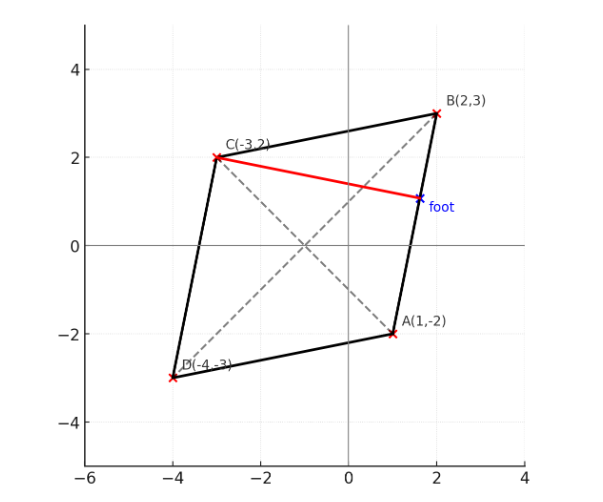
\includegraphics[width=0.8\columnwidth]{figs/fig4.png}
\end{center}

\end{document}

